\documentclass[11pt]{article}
\usepackage[a4paper,margin=20mm]{geometry}
\usepackage{amsmath,booktabs,graphicx}
\setlength{\parindent}{0pt}
\setlength{\parskip}{5pt}
\begin{document}
\section*{Measured reuse of HNL--MAC interaction lists}

The experiment uses $N=100\,656$, $p=6$, $P=4$,
$\theta=0.5$, and 64 CPU threads.  The density changes according to
$V_k=V_0+0.5(0.8)^kV_1$, while the mesh, targets, and MAC threshold remain
fixed.  In each of three independent 20-step runs, the control path actually
reconstructs the interaction lists at every step.  The reuse path retains the
initial lists.  Both paths share the same density update, moment construction,
and potential evaluation.  Every reconstructed near/far list agrees exactly
with the cached list.

\begin{table}[!htbp]
\centering
\caption{Median cumulative times over three runs.}
\begin{tabular}{rrrrrr}
\toprule
$K$ & Rebuild (s) & Reuse (s) & Saving (\%) & Speedup & Reuse/step (s)\\
\midrule
1  & 2.895  & 2.987  & $-3.1$ & 0.970 & 2.987\\
2  & 5.571  & 4.878  & 12.4   & 1.142 & 2.439\\
5  & 13.605 & 10.571 & 22.3   & 1.287 & 2.114\\
10 & 27.050 & 20.195 & 26.1   & 1.352 & 2.019\\
20 & 54.122 & 39.378 & 27.6   & 1.381 & 1.969\\
\bottomrule
\end{tabular}
\end{table}

\begin{figure}[!htbp]
\centering
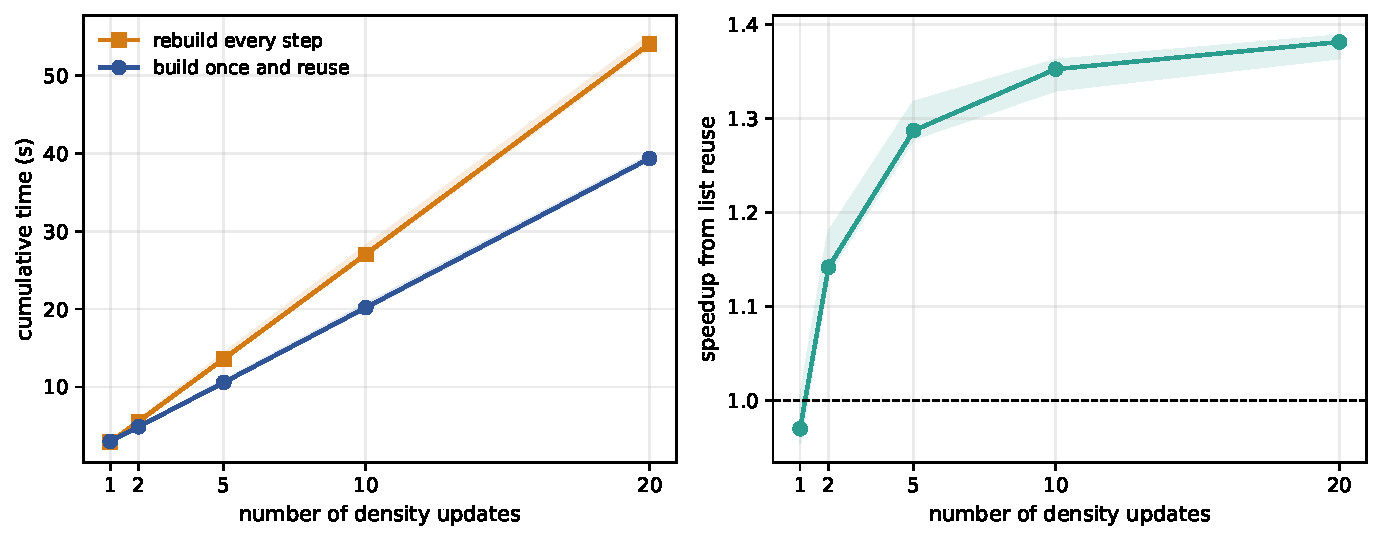
\includegraphics[width=0.88\textwidth]{list_reuse.pdf}
\caption{Cumulative time and speedup from interaction-list reuse.}
\end{figure}

The median per-step costs are 0.782~s for list reconstruction, 0.014~s
for updating source values, 0.124~s for moments, and 1.764~s for potential
evaluation.  Reuse therefore provides a clear but bounded benefit: after 20
updates it saves 27.6\% of cumulative time, while potential evaluation remains
the dominant cost.  This test isolates reuse on a frozen mesh and is not a
complete Kohn--Sham SCF calculation.
\end{document}
